\chapter{Dataset}\label{chap:Dataset}

% this chapter will discuss the existing whatever known words and yeah so obviously before delving you need to connect those two and it will compare the uh this si really weird the uh pros and cons but a sciency way adantages disadv only currently known datasets featuring real noise yeah as a introduction to uhm what's the word uhm idk to uknow describe how you made how and why the natural image noisy was made uknow to make it sound better does that kind of make sense

Chapter \ref{chap:Dataset} discusses the existing datasets that are relevant to the denoising problems and the \acl{NIND} provided with this work. The datasets presented in \acf{DND} and Renoir \cite{renoir} were created for benchmarking purposes and, as such, they outline the usefulness of a proper image noise dataset that may be used to train a denoising model in place of using synthetic noise. Other works provide paired datasets that are large enough to train a denoising model and the authors successfully demonstrate the performance of such models, but they were designed with specific applications in mind, namely cell-phone \cite{sidd} and low-light imaging \cite{learningtoseeinthedark}. We introduce the \acl{NIND} for general-purpose image denoising on images from conventional \ac{DSLR} and mirrorless cameras. Section \ref{sec:Natural Image Noise Dataset} describes the content of the \ac{NIND}, the complete acquisition process, and the steps needed for publication (because the dataset is open to contributions) and retrieval.

\section{Related work}
The following works feature datasets made of ground-truth / noisy image sets. The static scenes approach is necessary to directly compare the level of degradation using a loss function such as the \ac{SSIM} index or the \ac{MSE}. 
\subsection{Darmstadt Noise Dataset}
Synthetic noise is typically used to train and test models, but it had been unclear whether the reported synthetic results translated to real improvements. The \acl{DND}, containing 50 pairs of noisy-clean images from four cameras, was developed for the purpose of validating denoising algorithms using real data. Plötz and Roth showed that many modern denoising methods do not perform well on real data and that \ac{BM3D} \cite{bm3d}, which was published in 2006, remains one of the best performing methods \cite{darmstadt}. RENOIR \cite{renoir} is a similar dataset that was published prior to the \acs{DND}; however, Plötz and Roth noted spatial misalignments that reduced its effectivity. We have additionally found that the light sometimes differs between images in the same scene and that some photographs exhibit significant raw overexposure.
\subsection{Learning to See in the Dark}
\acf{SID} is an image noise dataset that is large enough for training and, to our knowledge, was used in the first successful attempt at denoising images using real image noise. This dataset focused on very low-light photography where the camera-generated JPEG appears black. The authors used a U-Net network architecture to create an end-to-end RAW-to-JPEG pipeline that produces realistic colors, improving on standard processing and \acs{BM3D} denoised images which still suffer from color bias at high ISO. Our work differs from \ac{SID} in that we aimed to train a general purpose (``blind") denoiser rather than one that handles a specific condition, such as extremely low light images. We chose to work in sRGB space because handling the whole RAW-to-sRGB pipeline removes some information which may otherwise be useful to the author during development. Moreover, one dataset can then be used with different types of color filter arrays.
%raw-to-srgb (cons: removes freedom of photographer)
\subsection{Smartphone Image Denoising Dataset}
The \acf{SIDD} is comprised of 10 scenes * 5 cameras * 4 conditions * 150 images, totalling 30000 images. This dataset aims to address the problem of smartphone image denoising, where the small sensor and aperture size causes noticeable noise even in pictures taken at base ISO. Further processing is thus applied to create ground-truth images out of many images. This method of creating ground-truth images is not entirely relevant for denoising images captured with larger sensors because a single image taken at base ISO on a DSLR-like camera is clean enough to work as ground-truth for training purposes.
%\subsubsection{Network architectures}
%
%We initially trained a DnCNN\cite{dncnn} architecture which is 
%- rednet (and dncnn)
%- U-Net
% This probably doesn't belong here
\section{Natural Image Noise Dataset}\label{sec:Natural Image Noise Dataset}

%\marginpar{DRAFTy-as-heck sentence}
The \acf{NIND} fills the gap for an image noise dataset of ground-truth - noisy image sets that targets cameras equipped with larger sensors\footnoteref{largesensornote} and which is large and varied enough (in both noise values and content types) to train a denoising model for ISO-blind denoising.%\marginpar{FIXME long run-on sentence}

Here we outline the physical setup required to capture image sets for the \ac{NIND}, summarize its content, explain the software processing and validation requirements, and describe its publication aspects such that others that wish to do so may also contribute.
\subsection{Capture}
We captured several images per static scene; at least one ground-truth taken with the camera's lowest ISO setting and several images taken with increasing ISO settings and consequent decreasing shutter speed in order to match the original exposure value. Scenes were captured using a camera affixed to a tripod and controlled with a wireless remote control to avoid shifting the setup position. We ensured that the ground was stable, wind would not cause any change in the scene, lighting did not vary between shots, and no area was overexposed in the ground-truth images. Overexposure occurs when the sensor is saturated. On a ground-truth image this would potentially benefit the high ISO images because less light is captured with a faster shutter speed; therefore, the higher ISO images may not be overexposed and thus may contain detail that is not present in the overexposed ground-truth. The aperture remained the same on all shots and the focus was set manually so that it would not automatically adjusted for each frame.

A base ISO image (ISO200 on the \acl{X-T1}) was always taken at least once, along with the camera's highest ISO setting (ISO6400 on the \acs{X-T1}). Several images were taken with different intermediate ISO values such that the ISO settings varied across each scene. We often also took images that we categorized as ``High ISO," which consisted of the highest ISO value and increased shutter speed. ``High ISO" images result in dark frames which are then correctly exposed using software. We often tried to match shutter speeds that would be useful to denoise, such as 1/60 s for handheld photography, 1/15 s for devices equipped with optical image stabilization, and 1/1000 s or faster for high-speed photography. We ensured that every ISO value was well represented in order to train models effective at blind denoising. On average, six images were produced per scene and some scenes featured multiple ground truth images which could be used in training to help prevent over-fitting.
\subsection{Content}

\begin{table}
\caption{Content of the Natural Image Noise Dataset}
%\centering
\resizebox{1\linewidth}{!}{
\begin{tabular}{lllllllllllllllllll|ll}
\ul{ISO value} & \ul{100} & \ul{200} & \ul{250} & \ul{320} & \ul{400} & \ul{500} & \ul{640} & \ul{800} & \ul{1000} & \ul{1250} & \ul{1600} & \ul{2000} & \ul{2500} & \ul{3200} & \ul{4000} & \ul{5000} & \ul{6400} & \ul{High} & \ul{Scenes} & \ul{Images} \\
\ul{Fujifilm X-T1}      &           & 105       & 11        & 8         & 18        & 13        & 16        & 25        & 16         & 9          & 12         & 9          & 19         & 25         & 17         & 19         & 91         & 123        & 90         & 536          \\
\ul{Canon C500D}     & 14        & 10        &           &           & 10        &           &           & 10        &            &            & 9          &            &            & 11         &            &            &            & 10         & 11         & 74           \\ \hline
\ul{Total}     & 15        & 116       & 11        & 8         & 29        & 13        & 16        & 36        & 16         & 9          & 22         & 9          & 19         & 37         & 17         & 19         & 91         & 133        & 101        & 616         
\end{tabular}%
}

% \vspace{-0.2cm} 
\label{tableDSContent}
\end{table}

\begin{figure}
%\centering
%\fbox{\rule{0pt}{2in} \rule{.9\linewidth}{0pt}}
  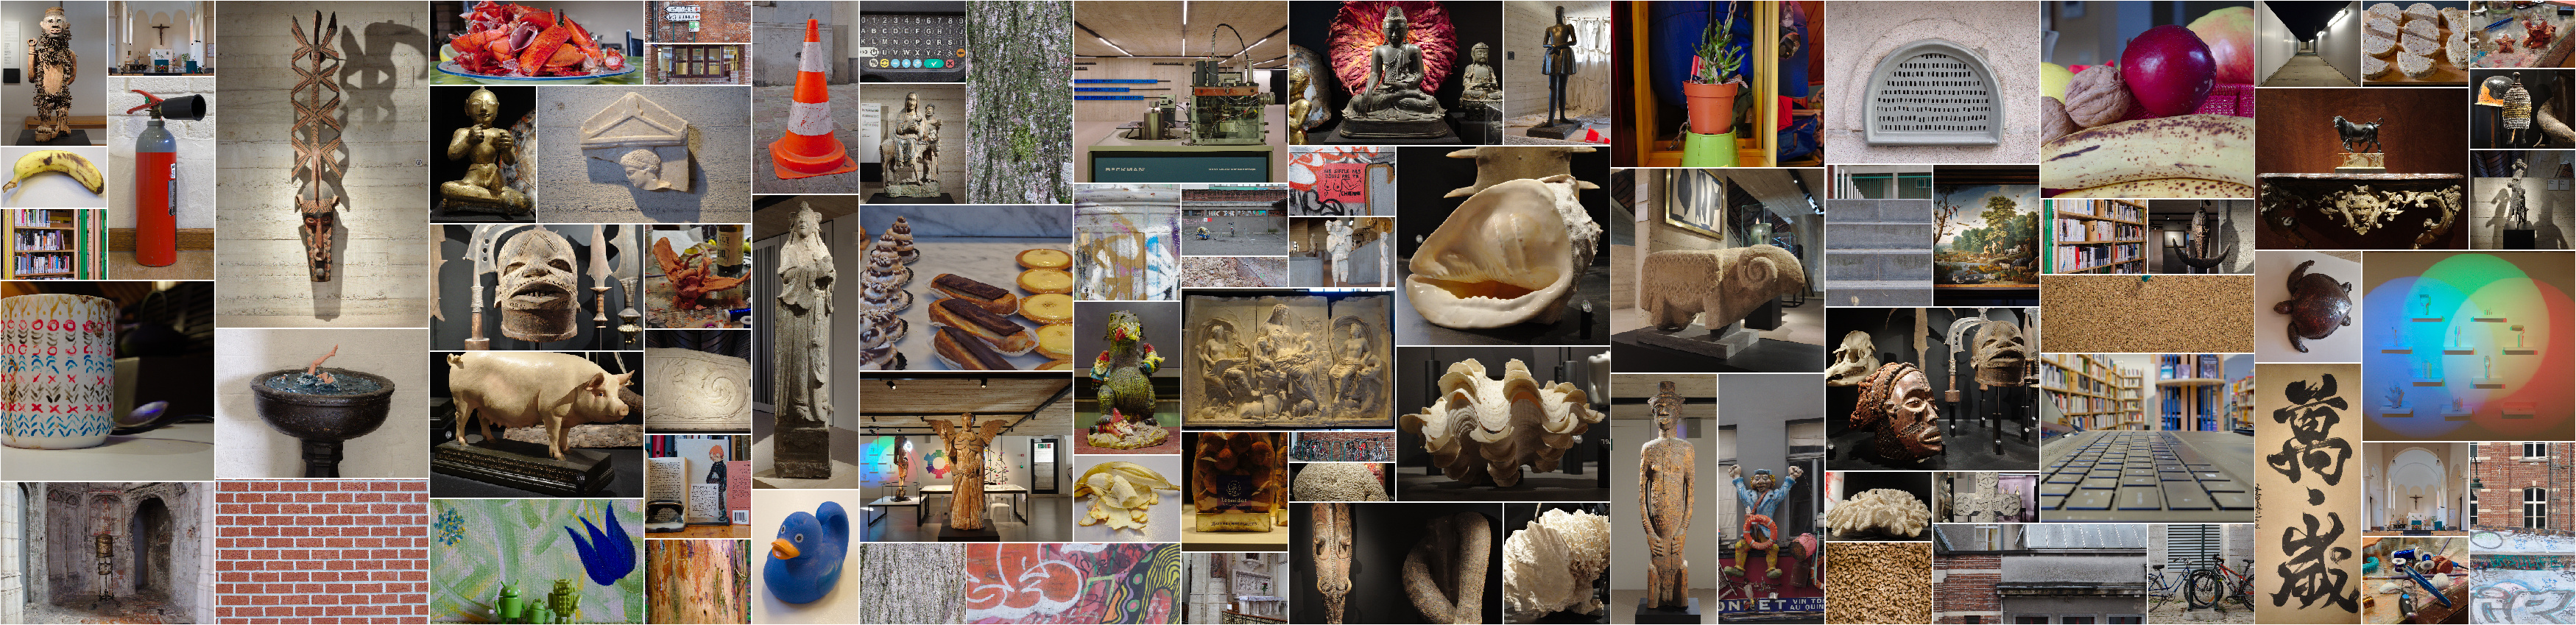
\includegraphics[width=1\linewidth]{gfx/samplebanner.jpg}
   \caption{Sample ground-truth images from the Natural Image Noise Dataset.}
%\vspace{-0.2cm} 
\label{fig:sampleimg}
\end{figure}

% TODO compute noise value on these
Many objects were captured in museums where subjects are plentiful (albeit we had to be mindful of copyright restricted material) and for which a denoising application would be highly relevant because indoor handheld pictures require a high ISO sensitivity. However, initial tests found that using images taken only indoors did not provide the variety needed to create a model that generalized well across all conditions, as natural colors were sometimes off in outdoor and brightly lit applications. We thus captured natural objects with vibrant colors (such as food items and plant-life) as well as outdoor scenes where the shutter speed could be taken as fast as 1/13000 s using a digital shutter. We made an effort to include some text because it is prevalent, yet we expect a model would not be able to guess how to reconstruct it, and we tried to make the images pleasant to look at in order to enhance the time users would spend looking at them. Most of the NIND images were captured on a \acl{X-T1} mirrorless camera, which uses a 23.6 x 15.6 mm X-Trans sensor. A \ac{C500D}, featuring a 22.3 x 14.9 mm standard Bayer sensor, was used to capture images that could be used to validate the generalization. The content of the dataset is summarized in Table \ref{tableDSContent} and a subset of the \acs{X-T1} pictures are shown in Figure \ref{fig:sampleimg}.
\subsection{Software processing}
We processed the dataset images using darktable \cite{darktable} (an open source development software) for raw-to-sRGB development. Our development steps are similar to those we would apply to a standard picture but no sharpening was applied, as this greatly amplifies noise and is typically applied last in the pixel pipeline (we can expect users to apply sharpening to the generated clean image without any perceptible loss). We used darktable's automatic exposure mode to match a fixed percentile target on the histogram and calculate the required exposure compensation for all images in a set. Likewise, we ensured that the white balance was identical and all development steps were copied over to the entire scene. (The exposure percentile and white balance settings are fixed within a scene but vary across different scenes.) The raw overexposed indicator was used to verify that no overexposed areas were present in the base ISO image and if any were detected then it was cropped out or the scene was discarded. The images were visually inspected to detect slight variations in light, the introduction of foreign objects such as insects, or any movement, which also resulted in cropping or discarding images. The ground-truth images must be at least as sharp as their noisy counterparts; this is sometimes not the case due to slight movements on longer exposures. The remaining images were saved in either high-quality (98 to 100) 8-bit JPEG or lossless 16-bit PNG.

The last step of development is to use Hugin's align\_image\_stack tool \cite{hugin} to ensure that all images in a set are perfectly pixel-aligned. The tool will usually return the same image size as the input, in which case the whole image set can safely be used. When a difference is detected then the tool will automatically align the set and we visually analyzed whether the result was acceptable or the movement caused a change in perspective, in which case the outlier images were discarded. Some noisy images cannot easily be matched to the scene; possible solutions are to denoise these images in order to check the alignment or to take a cleaner image afterward and assume that the middle images are consistent with the previous and next ones.
\subsection{Publishing}
The Natural Image Noise Dataset is published on Wikimedia Commons ( \url{https://commons.wikimedia.org/wiki/Natural_Image_Noise_Dataset} ), an online repository of free-use images and other digital media. Wikimedia Commons hosts media content for all Wikimedia projects and its scope is limited only by the content having some educational value (broadly meaning ``providing knowledge; instructional or informative"). As such, we believe it is a fitting platform for the publication of a research dataset.

One key advantage of using Wikimedia Commons is its collaborative aspect. Anyone is allowed to add images to the dataset, modify existing images (for example to fix a spatial misalignment), and discuss the content (through the discussion page provided for each file, category, and the dataset itself). The collaborative aspect also includes a ``Quality images candidates" page \cite{qic} where users assess the technical quality of a submitted image and may promote it to a ``Quality image" standing. Many of the ground-truth images have gone through this process and were promoted through human assessment. The same process was also used to validate the trained model, which ended up in a positive assessment since even the denoised dynamic ISO6400 picture presented in Figure \ref{fig:visualpigeons} was among the promoted images.

On the technical side, Wikimedia Commons preserves images as they are uploaded; JPEG images are not recompressed, 16-bit lossless TIFF and PNG images are allowed, and the metadata is kept. Thumbnails are generated and images may be visualized before being downloaded in full resolution, and the download may include a select subset instead of the whole dataset. A customizable download script is provided on the dataset's page for convenient retrieval. Even though files can be overwritten, every file uploaded on Wikimedia Commons is kept forever therefore specific snapshots of the dataset can be made and the download script can fetch the dataset as it was on any specified date.

It is also important to note the usefulness of the data outside of a denoising dataset context. Many images, such as those depicting artifacts displayed in churches and museums, have encyclopedic value and the ground-truth images present in our dataset are of higher quality than most previously available images depicting such artifacts. By publishing the dataset on Wikimedia Commons, these ground-truth images may be used in Wikipedia articles directly\footnote{E.g. \href{https://en.wikipedia.org/wiki/Bobo_people}{Bobo people}, \href{https://en.wikipedia.org/wiki/Bombardment_of_Brussels}{Bombardment of Brussels}, \href{https://en.wikipedia.org/wiki/Dengese_people}{Dengese people}}. This may be a motivating factor to those wishing to contribute.
